% =====================================================================
%  2026-05-12 — Pico 焊接、最終電路定稿、決定 fork C++ 版本
% =====================================================================

\subsection*{今日目標}

\begin{itemize}[leftmargin=2em,itemsep=0pt]
  \item 5/11 取的 \textbf{HS-02A 烙鐵}今天正式上戰場:
        \textbf{Pico 排針焊上}、\textbf{BPW34 焊成獨立長線},麵包板可以乾淨收線。
  \item 把 \textbf{74HC4051 MUX} 接到四檔 \(R_F\) (5/11 採購)、串到 op-amp 反相輸入、
        S0/S1 從 Pico GPIO 控,真正把「四檔自動換」這條線跑起來。
  \item 把整塊電路收成\textbf{最終定稿}:單一 Type-C 供電、OLED 接上、感測器與電路分離。
  \item 開始調 mux 自動換檔的 hysteresis 狀態機(5/11 那個 insight 的程式化)。
  \item \textbf{下一個分水嶺}:調著調著發現 MicroPython 採樣速度撐不住目標,
        正式 fork 一個 \textbf{C++ Pico SDK 版本}的 firmware 走下去。
\end{itemize}

\subsection*{第一個任務:焊接}

\paragraph{Pico 排針。} 5/11 採購的 Pico(20-pin \(\times 2\))出廠時排針是分離的;
今天用 HS-02A(C245 系統,330 \(^\circ\)C)把 40 隻腳焊上 \(\approx\) 15 分鐘搞定。
焊錫筆 \(\SI{1.0}{\milli\metre}\) 配無鉛助焊劑(松香膏),焊點圓潤、無短路。

\paragraph{BPW34 焊長線。} 5/6 量測的痛點之一是 BPW34 翹起來、貼不到螢幕。
今天用 \(\sim 30\) cm 帶絕緣的雙芯細線把 BPW34 與麵包板分開,
末端焊接點熱縮管包好(圖~\ref{fig:0512-bpw34}),BPW34 就能像「探棒」一樣\textbf{平貼螢幕}量測。

\begin{figure}[H]
  \centering
  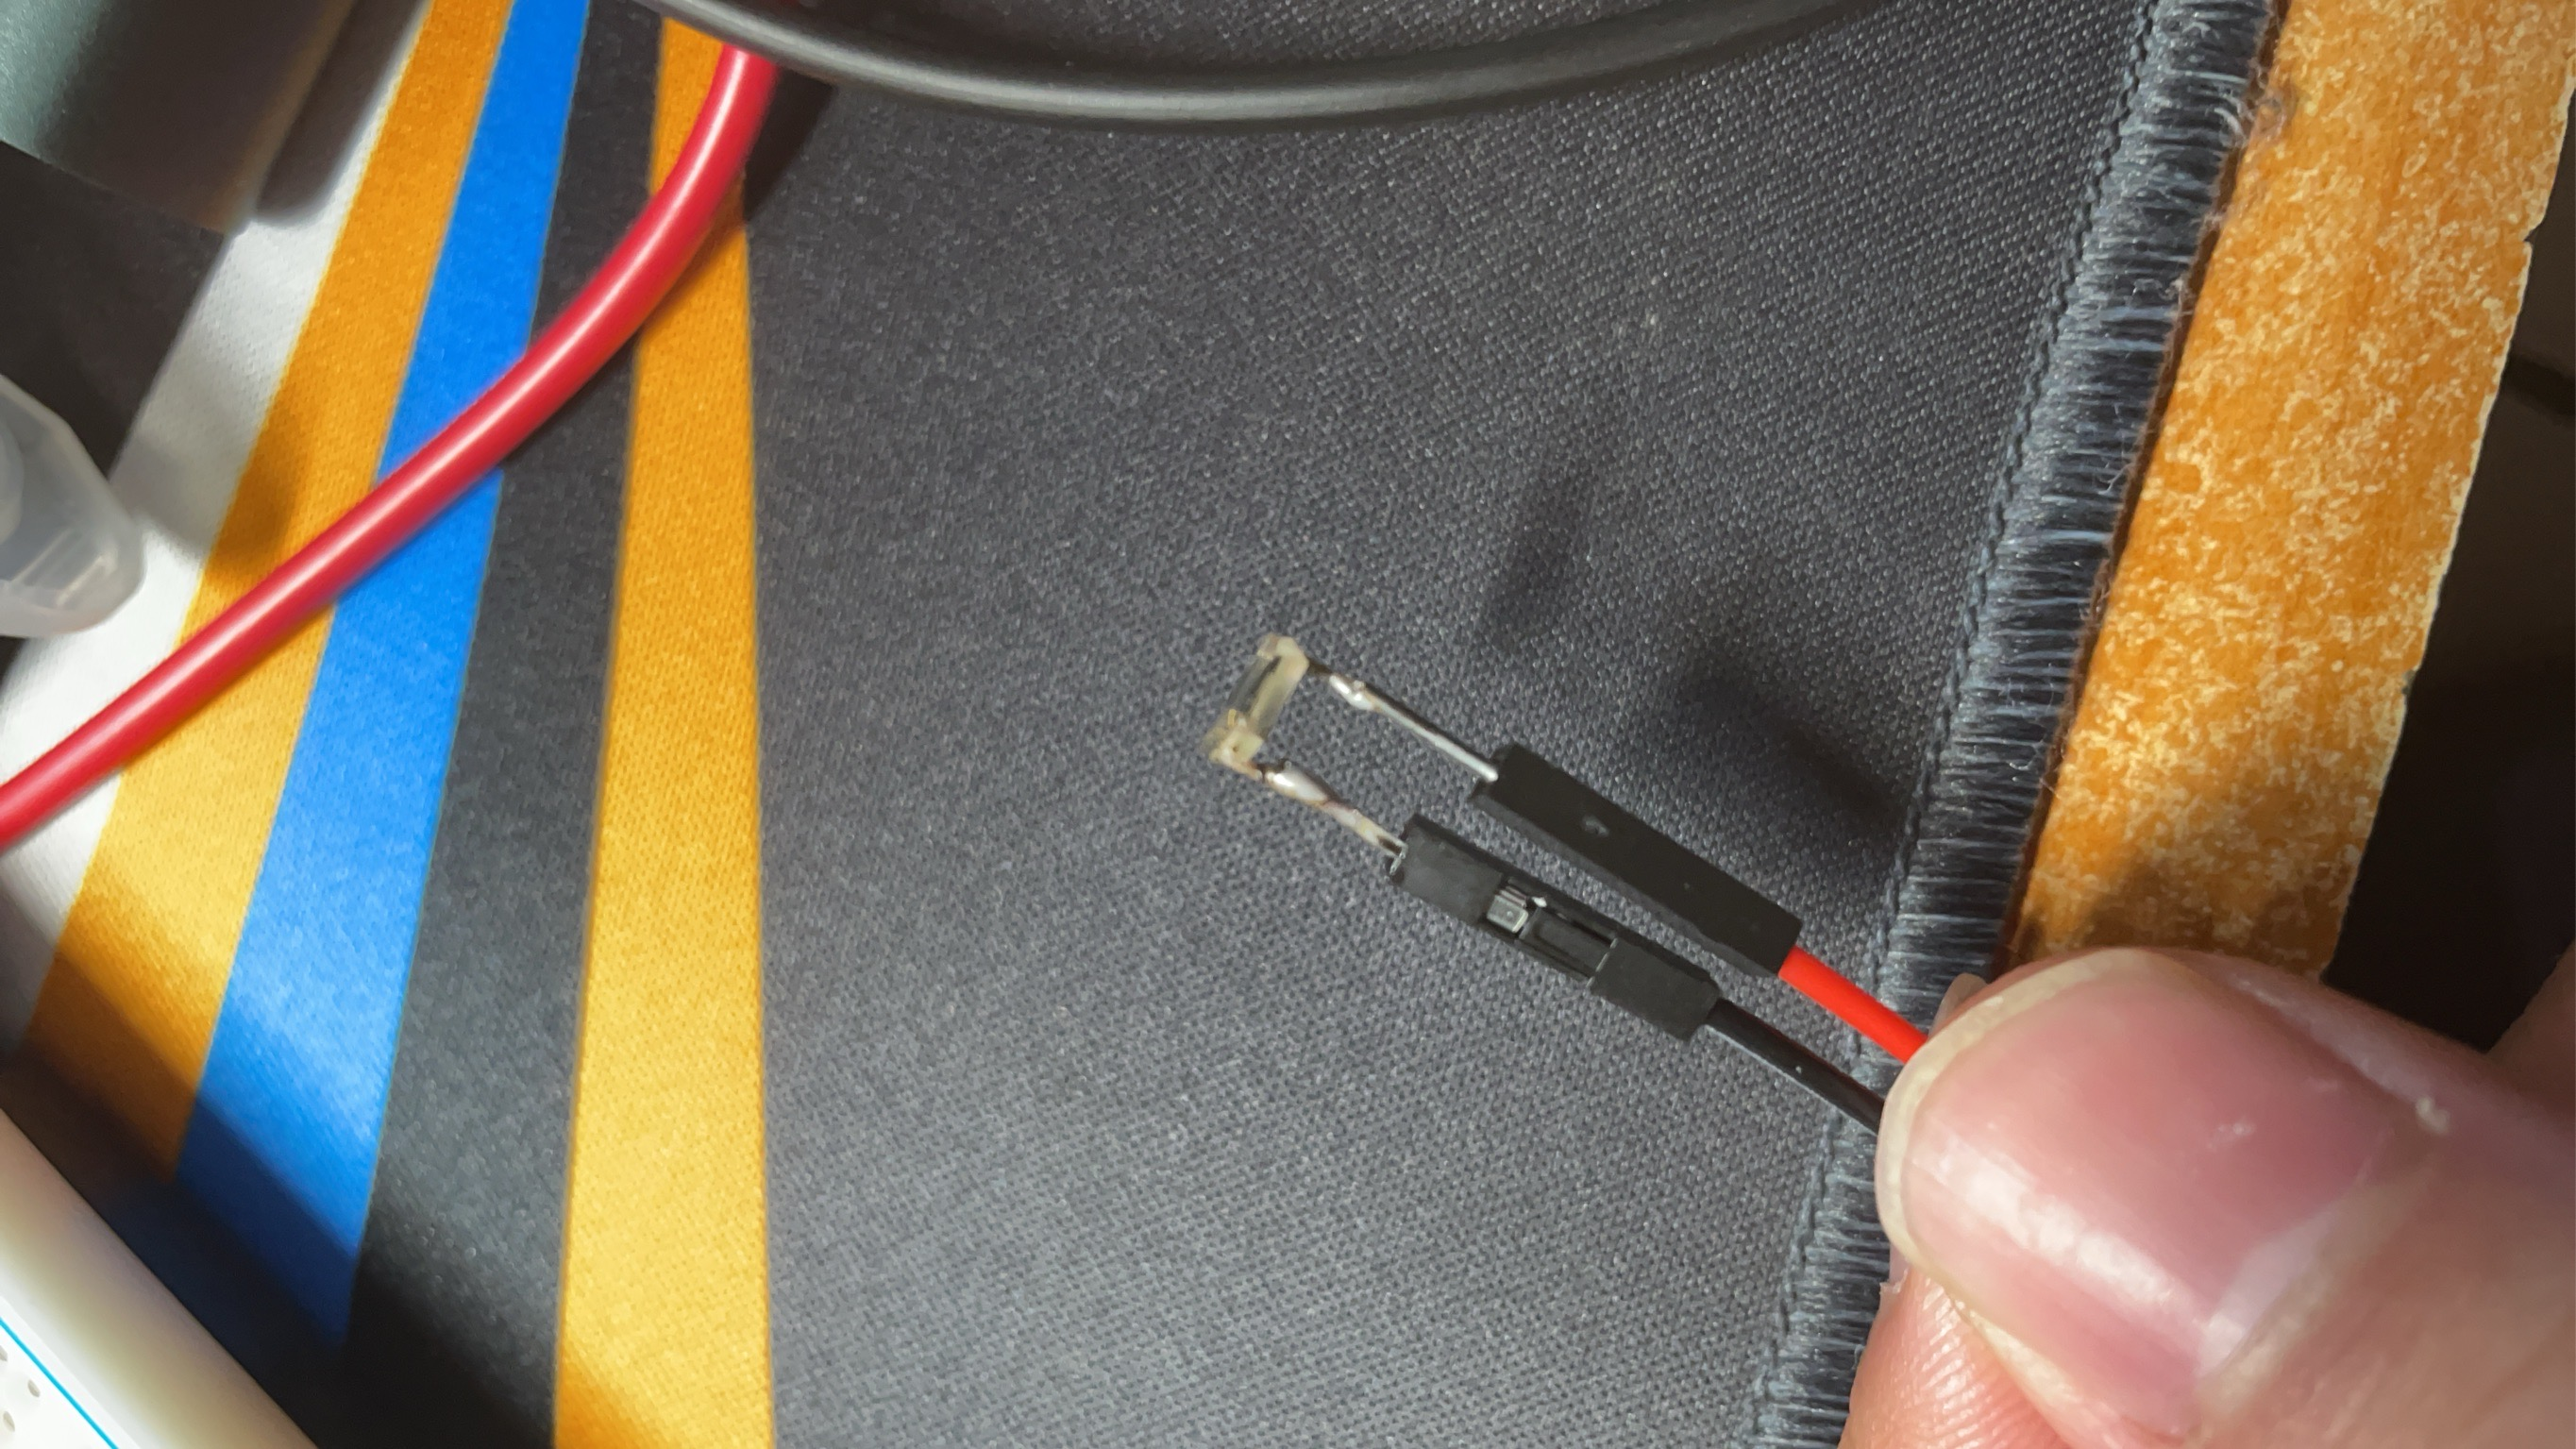
\includegraphics[width=0.55\linewidth]{2026-05-12/BPW34_solder.JPG}
  \caption{BPW34 焊到 30 cm 雙芯線末端,根部熱縮管固定,
           長線設計讓感測器可以離開麵包板平貼待測螢幕。}
  \label{fig:0512-bpw34}
\end{figure}

\subsection*{第二個任務:把 74HC4051 接到四檔 \(R_F\)}

5/11 從 Gemini 借來的拓樸今天落地:

\begin{itemize}[leftmargin=2em,itemsep=0pt]
  \item \texttt{COM}(Z 腳)接 op-amp 反相輸入(MCP6004 Pin 2)
  \item \texttt{Y0/Y1/Y2/Y3} 各接一支 \(R_F\):1 kΩ / 10 kΩ / 100 kΩ / 1 MΩ
  \item \(R_F\) 另一端統一拉到 op-amp 輸出(Pin 1)
  \item \texttt{S0/S1} 各接 Pico GPIO 一隻,\texttt{S2} 拉地(用不到第 5--8 通道)
  \item \texttt{INH}(enable, low-active)拉地長期開
\end{itemize}

\subsection*{第三個任務:電路最終定稿}

把零件擺位收成圖~\ref{fig:0512-final}的版本,有四個明顯升級:

\begin{enumerate}[leftmargin=2em,itemsep=2pt]
  \item \textbf{沒有杜邦線繞成一坨} —— 5/11 採購的 140 根預剪硬跳線終於發揮 ——
        所有走線水平貼板,目視能直接 trace 訊號流。
  \item \textbf{BPW34 從電路獨立出去} —— 透過上面那條 30 cm 長線拉出來,
        貼螢幕量測不會把整塊麵包板一起搬。
  \item \textbf{0.91" SSD1306 OLED 完整驅動} —— I\textsuperscript{2}C 兩線從 Pico 接出來,
        \texttt{firmware/python-version/ssd1306.py} (5/11 寫好) 直接吃。
  \item \textbf{全部單一 Type-C 供電} —— Pico 的 USB-C 同時兼任電源 + 資料線,
        9V 變壓器 + MB-102 退役(那兩件先留著當實驗室備援電源)。
\end{enumerate}

\begin{figure}[H]
  \centering
  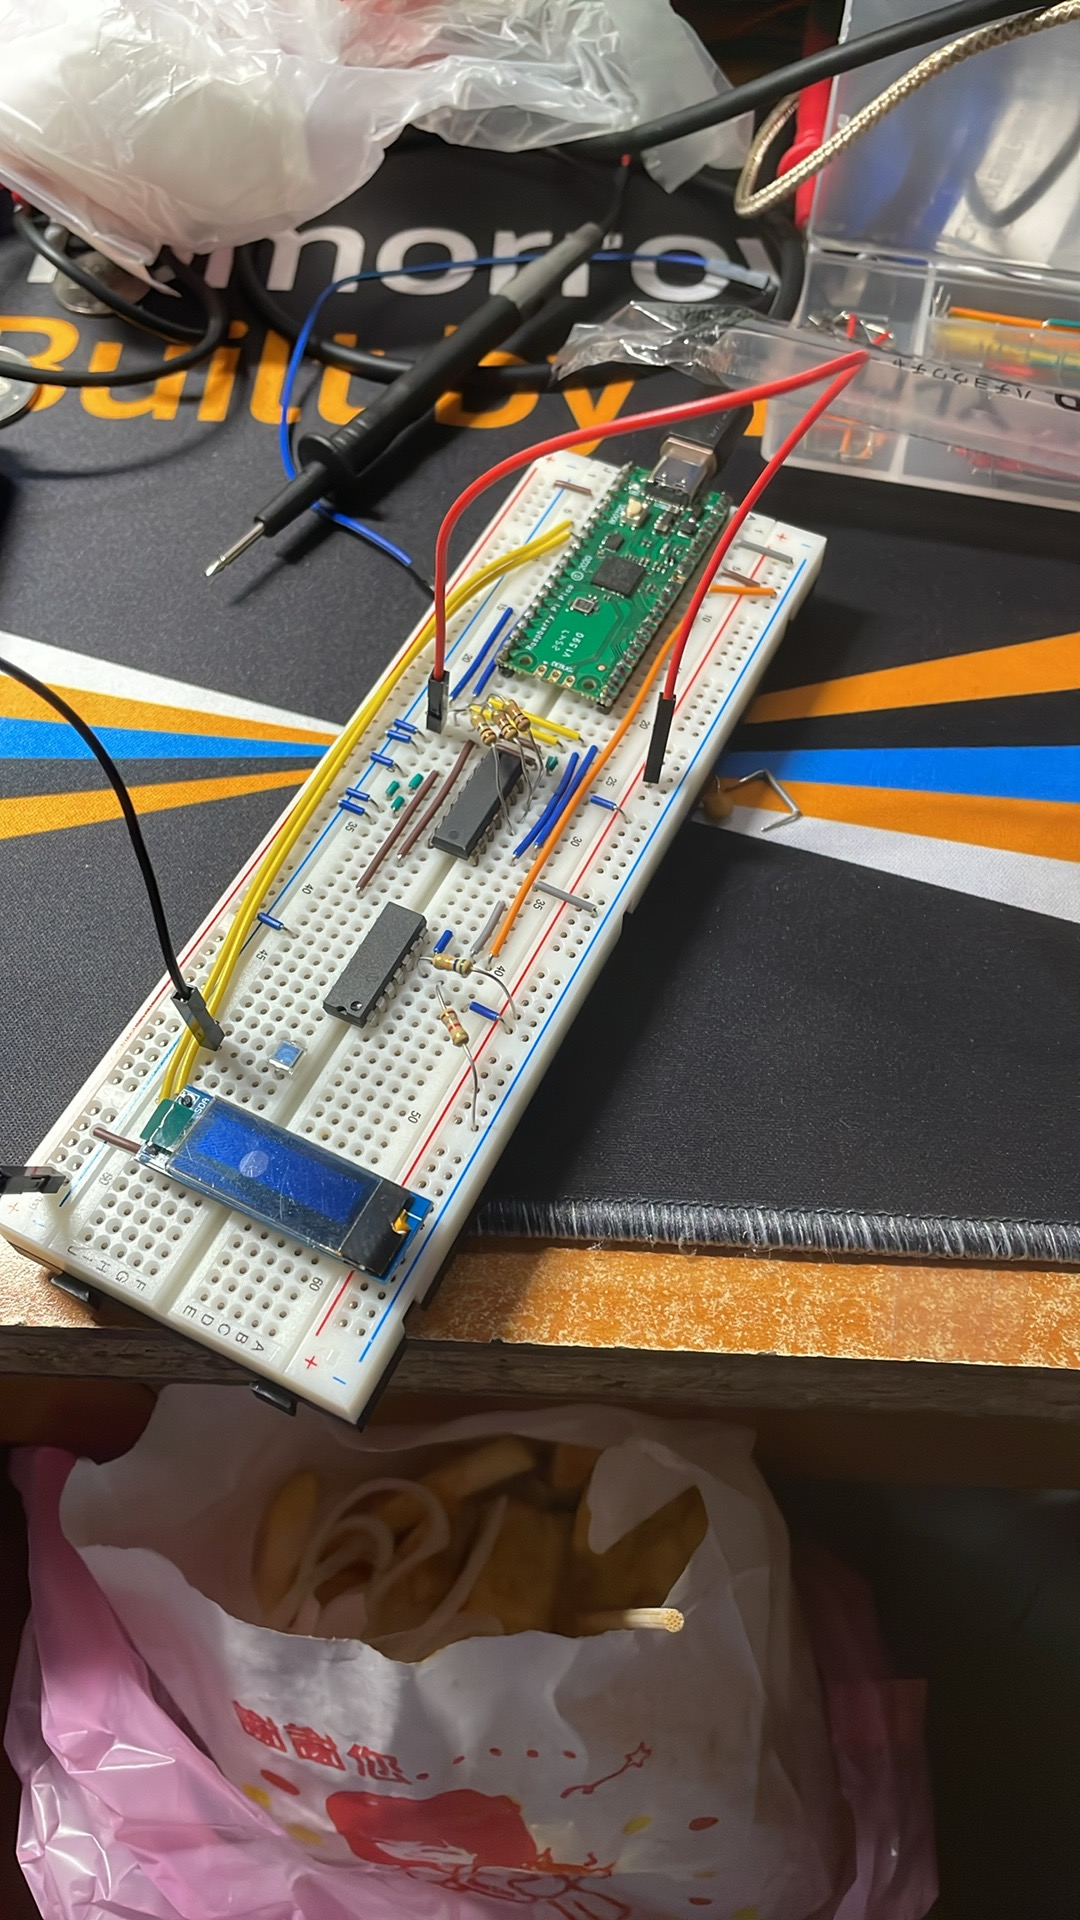
\includegraphics[width=0.85\linewidth]{2026-05-12/final_schmatic.JPG}
  \caption{2026-05-12 麵包板最終定稿:單 Type-C 供電(右下 Pico)、
           74HC4051 MUX + 四檔 \(R_F\)、MCP6004 TIA、SSD1306 OLED、
           BPW34 透過長線拉出畫面外平貼螢幕。}
  \label{fig:0512-final}
\end{figure}

\subsection*{第四個任務:hysteresis 自動換檔狀態機}

5/11 寫過構想了,今天程式化。MicroPython 端:

\begin{itemize}[leftmargin=2em,itemsep=0pt]
  \item 每 \(N\) 個樣本(目前 \(N = 100\),約 \(\SI{10}{\milli\second}\)) 算一次 mean。
  \item 若 mean \(> V_\text{HI} = \SI{2.8}{\volt}\) 連續 3 個視窗 \(\to\) 切下一檔較低 \(R_F\)。
  \item 若 mean \(< V_\text{LO} = \SI{0.5}{\volt}\) 連續 3 個視窗 \(\to\) 切下一檔較高 \(R_F\)。
  \item 切檔後 \(\SI{50}{\milli\second}\) cooldown(74HC4051 \texttt{tPHL}+RC settle 留 margin),
        cooldown 期間用 \texttt{print("\# GAP=...")} 通知 PC 端不要把這段當訊號。
\end{itemize}

實測:\textbf{會切,但切完抖一下}——cooldown 設太短 + MicroPython GC 時不時跳出來吃 50--100 ms,
換檔當下 PC 端能看到 burst-noise。可以調 cooldown 改善,但更基本的問題在後面那一節。

\subsection*{分水嶺:為什麼今天決定 fork C++ 版本}

調 mux 切檔時注意到幾個 MicroPython 撐不住的點:

\begin{itemize}[leftmargin=2em,itemsep=0pt]
  \item \textbf{ADC 取樣速率上限}:輪詢 \texttt{adc.read\_u16()} +
        \texttt{sys.stdout.write()} 兩件事就吃光 CPU,實測穩定上限 \(\approx \SI{8}{\kilo\hertz}\),
        距離 OLED PWM \(\SI{20}{\kilo\hertz}\) 要的 \(\geq 5 \times f\) Nyquist margin 不夠。
  \item \textbf{Jitter 大}:MicroPython runtime 不時 GC,\(\SI{50}{\micro\second}\) 級的 sample period
        會被偶發拉到 \(\SI{1}{\milli\second}\)+,FFT 出來有 sidelobe。
  \item \textbf{GAP marker 太頻繁}:OLED refresh、GC、切檔三個事件加起來,
        每秒會吐 5--10 個 GAP,PC 端拼時間軸要做太多 patch。
\end{itemize}

決定:\textbf{firmware 主線轉 C++ Pico SDK},用 PIO + DMA 把 ADC 取樣丟到 ring buffer,
GPIO 與 OLED I\textsuperscript{2}C 由 core1 慢工負責,采樣不再被任何 housekeeping 打斷。
MicroPython 版本保留在 \texttt{firmware/python-version/} 當原型參照,不丟。

\paragraph{cpp-version 目錄結構建好。}
\(\)同步把 C++ 兩個子專案的骨架擺進來,等接下來幾天慢慢長:

\begin{itemize}[leftmargin=2em,itemsep=0pt]
  \item \texttt{firmware/led-light-test-cpp-version/} —— C 版本的 blink
        (\texttt{blink.c} + \texttt{CMakeLists.txt} + \texttt{pico\_sdk\_import.cmake}),
        對應 python-version 的 blink.py;\textbf{確認 Pico SDK 編譯鏈通了}的基準起點。
  \item \texttt{firmware/cpp-version/} —— flicker meter 主程式 C++ 骨架
        (\texttt{main.cpp} + \texttt{ssd1306.cpp/.hpp} + 自家 SSD1306 OLED 驅動 +
        CMake build system)。今天先把目錄 + 起手檔 commit 起來,
        ADC PIO/DMA 那塊明後天動。
\end{itemize}

\subsection*{今日心得}

\begin{itemize}[leftmargin=2em,itemsep=0pt]
  \item \textbf{MicroPython 是好原型,但不是好量產}。功能完整跑通(blink \(\to\) ADC \(\to\) OLED \(\to\)
        mux \(\to\) 自動換檔)花了 4 天(5/8\,\(\to\)\,今天),效能瓶頸碰到要轉 C++ 也是 4 天。
        快速失敗才能快速知道接下來要走哪條路。
  \item \textbf{把語言版本當成資料夾並排}的設計(\texttt{python-version/} \(+\) \texttt{cpp-version/})
        現在看格外划算 —— python-version 不用刪、可繼續當原型 sandbox,cpp-version 主線重寫。
        日後甚至可以做兩版的同電路對比(同一 ADC 訊號 \(\to\) 兩個版本各跑 FFT \(\to\) 誰的 jitter 小)。
  \item \textbf{下一步}:
        \begin{enumerate}[leftmargin=2em,itemsep=0pt]
          \item C++ 端把 ADC \(\to\) PIO \(\to\) DMA \(\to\) ring buffer 那條鏈寫完,
                目標 \(\SI{100}{\kilo\hertz}\) 採樣率穩定無 jitter。
          \item OLED 從 C++ 端重新驅動(\texttt{ssd1306.cpp/.hpp} 已起手),
                跟 \texttt{firmware/python-version/ssd1306.py} 行為對齊。
          \item PC 端 \texttt{host/read\_data.py} 已能吃 binary 三 byte frame + GAP marker,
                C++ 版本只要照協定吐就能直接接,Host 不用動。
        \end{enumerate}
\end{itemize}
